\documentclass[aspectratio=169,10pt]{beamer}
\usetheme{Madrid}
\usecolortheme{seahorse}
\setbeamertemplate{navigation symbols}{}

\usepackage{amsmath,amssymb,mathtools}
\usepackage{booktabs}
\usepackage{graphicx}
\usepackage{tabularx}
\usepackage{siunitx}
\usepackage{xcolor}

\definecolor{DeepBlue}{HTML}{0B2C4A}
\definecolor{DeepTeal}{HTML}{0F766E}
\definecolor{WarmGold}{HTML}{B45309}
\definecolor{SoftGray}{HTML}{F4F6FA}

\setbeamercolor{title}{fg=white,bg=DeepBlue}
\setbeamercolor{frametitle}{fg=white,bg=DeepBlue}
\setbeamercolor{structure}{fg=DeepBlue}
\setbeamercolor{block title}{fg=white,bg=DeepTeal}
\setbeamercolor{block body}{bg=SoftGray}
\setbeamercolor{itemize item}{fg=DeepTeal}

\setbeamertemplate{footline}{
  \leavevmode%
  \hbox{%
    \begin{beamercolorbox}[wd=.80\paperwidth,ht=2.5ex,dp=1.0ex,leftskip=1.2em]{author in head/foot}%
      \usebeamerfont{author in head/foot}MEAM4600 Final Project: Posterior Projection Study
    \end{beamercolorbox}%
    \begin{beamercolorbox}[wd=.20\paperwidth,ht=2.5ex,dp=1.0ex,center]{date in head/foot}%
      \insertframenumber/\inserttotalframenumber
    \end{beamercolorbox}%
  }%
}

\title{Projection Schedule \& Order Study}
\subtitle{Inverse Posterior Sampling for 1D Nonlinear Elliptic PDE}
\author{Final Project Summary}
\date{2026-04-22}

\begin{document}

\begin{frame}
  \titlepage
\end{frame}

\begin{frame}{Project Completion Check}
\begin{block}{Status vs Initial Plan}
\begin{itemize}
  \item Start point respected: standalone \texttt{meam4600\_final\_proj}, baseline commit \texttt{a0b111e}.
  \item Integrity check passes: \texttt{PYTHONPATH=src .venv/bin/python -m unittest discover -s tests} (\textbf{15/15}).
  \item Dataset available: \texttt{data/chonkdiff\_elliptic\_dataset.npz}.
  \item Baseline and tuned checkpoints/evaluations completed, including full \(\mathbf{128 \times 3}\) ranking tables.
  \item Scientific deliverables done: objective winners, tradeoffs, and recommendation in \texttt{reports/final\_projection\_study\_summary.md}.
\end{itemize}
\end{block}
\vspace{0.3em}
\textbf{Conclusion:} the project is complete with respect to the declared acceptance criteria.
\end{frame}

\begin{frame}{Problem Setup and Mathematical Definition}
\small
We study inverse posterior sampling for:
\[
-\Delta v + \kappa v^3 = u, \qquad \kappa = 50,\quad x\in[0,1),\quad v(x+1)=v(x).
\]
Discretization (\(N_x=63\), \(\Delta x=1/N_x\), periodic indexing):
\[
(-\Delta_h v)_i = \frac{2v_i-v_{i-1}-v_{i+1}}{\Delta x^2},\qquad
r_i(u,v) = (-\Delta_h v)_i + \kappa v_i^3 - u_i.
\]
Inverse setting:
\[
\text{given }(m_i,\,v_i^{\mathrm{obs}}),\ \text{recover full }u \text{ (and consistent }v\text{)},
\]
where \(m_i\in\{0,1\}\) is a random observation mask (\(10\%\) observed fraction).
\end{frame}

\begin{frame}{Experimental Protocol and Parameters}
\small
\begin{tabular}{@{}ll@{}}
\toprule
\textbf{Category} & \textbf{Setting} \\
\midrule
Benchmark backend & \texttt{chonkdiff} nonlinear elliptic oracle \\
Grid and physics & \(N_x=63\), \(L=1.0\), \(\kappa=50\), periodic BC \\
Dataset & train \(=896\), val \(=128\), seed \(=42\) \\
Observations & random mask, observed fraction \(=0.1\), noise std \(=0\) \\
Evaluation size & \(128\) samples \(\times\) \(3\) observation seeds \\
Projection schedules & \texttt{none, final\_only, every\_step, every\_2, every\_5, late\_only, adaptive\_residual} \\
Projection orders & \texttt{first\_order}, \texttt{gauss\_newton} (plus \texttt{none/none} case) \\
Best checkpoint family & \texttt{posterior\_projection\_e200\_big} (\(h=96,\ L=6,\ \text{modes}=20\)) \\
Winning sampling knobs & guidance \(g=16.0\), steps \(=100\) \\
\bottomrule
\end{tabular}
\end{frame}

\begin{frame}{Metrics (Exact Implementation)}
\small
\[
\mathrm{relL2}(a,b)=\frac{\lVert a-b\rVert_2}{\max(\lVert b\rVert_2,10^{-12})}.
\]
\[
\mathrm{obs\_error}=
\sqrt{
\frac{\sum_i m_i\left(\hat v_i^{\mathrm{norm}}-v_i^{\mathrm{obs}}\right)^2}
{\max\left(\sum_i m_i,1\right)}
}.
\]
\[
\mathrm{posterior\_quality}
= \mathrm{relL2}(u_{\mathrm{pre}},u^\star)
+ \mathrm{relL2}(v_{\mathrm{pre}},v^\star)
+ \mathrm{obs\_error}.
\]
\[
\mathrm{physical\_consistency}=\lVert r(u_{\mathrm{pre}},v_{\mathrm{pre}})\rVert_2,\quad
\mathrm{trajectory\_stability}=\sum_t\lVert x_t-x_t^{(\texttt{none/none})}\rVert_2^2.
\]
\[
\mathrm{runtime}=\text{total wall-clock sample time (seconds)}.
\]
\vspace{0.25em}
\footnotesize
All ranking metrics are minimized; \(u_{\mathrm{pre}},v_{\mathrm{pre}}\) are pre-final-cleanup states.
\end{frame}

\begin{frame}{Full Study Winners (\(128\times3\), all compared runs)}
\small
\begin{tabular}{@{}llll@{}}
\toprule
\textbf{Objective} & \textbf{Winning run} & \textbf{Schedule / Order} & \textbf{Value} \\
\midrule
posterior\_quality & \(e200\_big,\ g=16\) & \texttt{every\_5 / gauss\_newton} & \(3.1364\) \\
physical\_consistency & \(e200\_big,\ g=16\) & \texttt{every\_step / gauss\_newton} & \(3.59\times10^{-4}\) \\
runtime & baseline & \texttt{none / none} & \(0.6086\ \mathrm{s}\) \\
trajectory\_stability & baseline & \texttt{none / none} & \(0.0\) \\
\bottomrule
\end{tabular}

\vspace{0.5em}
\begin{block}{Best inverse-recovery row (minimum \(u\)-error)}
\textbf{Run:} \(e200\_big,\ g=16\), \textbf{case:} \texttt{every\_step / first\_order} \\
\(u\_error=1.5050,\ v\_error=0.9120,\ obs\_error=0.8126,\ posterior\_quality=3.2295,\ runtime=1.3741\ \mathrm{s}\).
\end{block}
\end{frame}

\begin{frame}{Improvement vs Baseline and Previous Best (\(g=10\))}
\small
\begin{tabular}{@{}lccc@{}}
\toprule
\textbf{Metric (best-\(u\) row)} & \textbf{Baseline} & \textbf{\(g=10\)} & \textbf{\(g=16\)} \\
\midrule
posterior\_quality & \(4.3679\) & \(3.4633\) & \(\mathbf{3.2295}\) \\
\(u\_error\) & \(1.9232\) & \(1.5484\) & \(\mathbf{1.5050}\) \\
\(v\_error\) & \(1.2944\) & \(1.0102\) & \(\mathbf{0.9120}\) \\
obs\_error & \(1.1504\) & \(0.9046\) & \(\mathbf{0.8126}\) \\
runtime [s] & \(\mathbf{0.7357}\) & \(1.3185\) & \(1.3741\) \\
\bottomrule
\end{tabular}

\vspace{0.5em}
\begin{itemize}
  \item \(g=16\) vs baseline: \(-21.75\%\) in \(u\_error\), \(-26.06\%\) in posterior\_quality, \(+86.77\%\) runtime.
  \item \(g=16\) vs \(g=10\): \(-2.81\%\) in \(u\_error\), \(-6.75\%\) in posterior\_quality, \(+4.21\%\) runtime.
\end{itemize}
\end{frame}

\begin{frame}{Guidance Trend: Quality Improves, Runtime Rises}
\centering
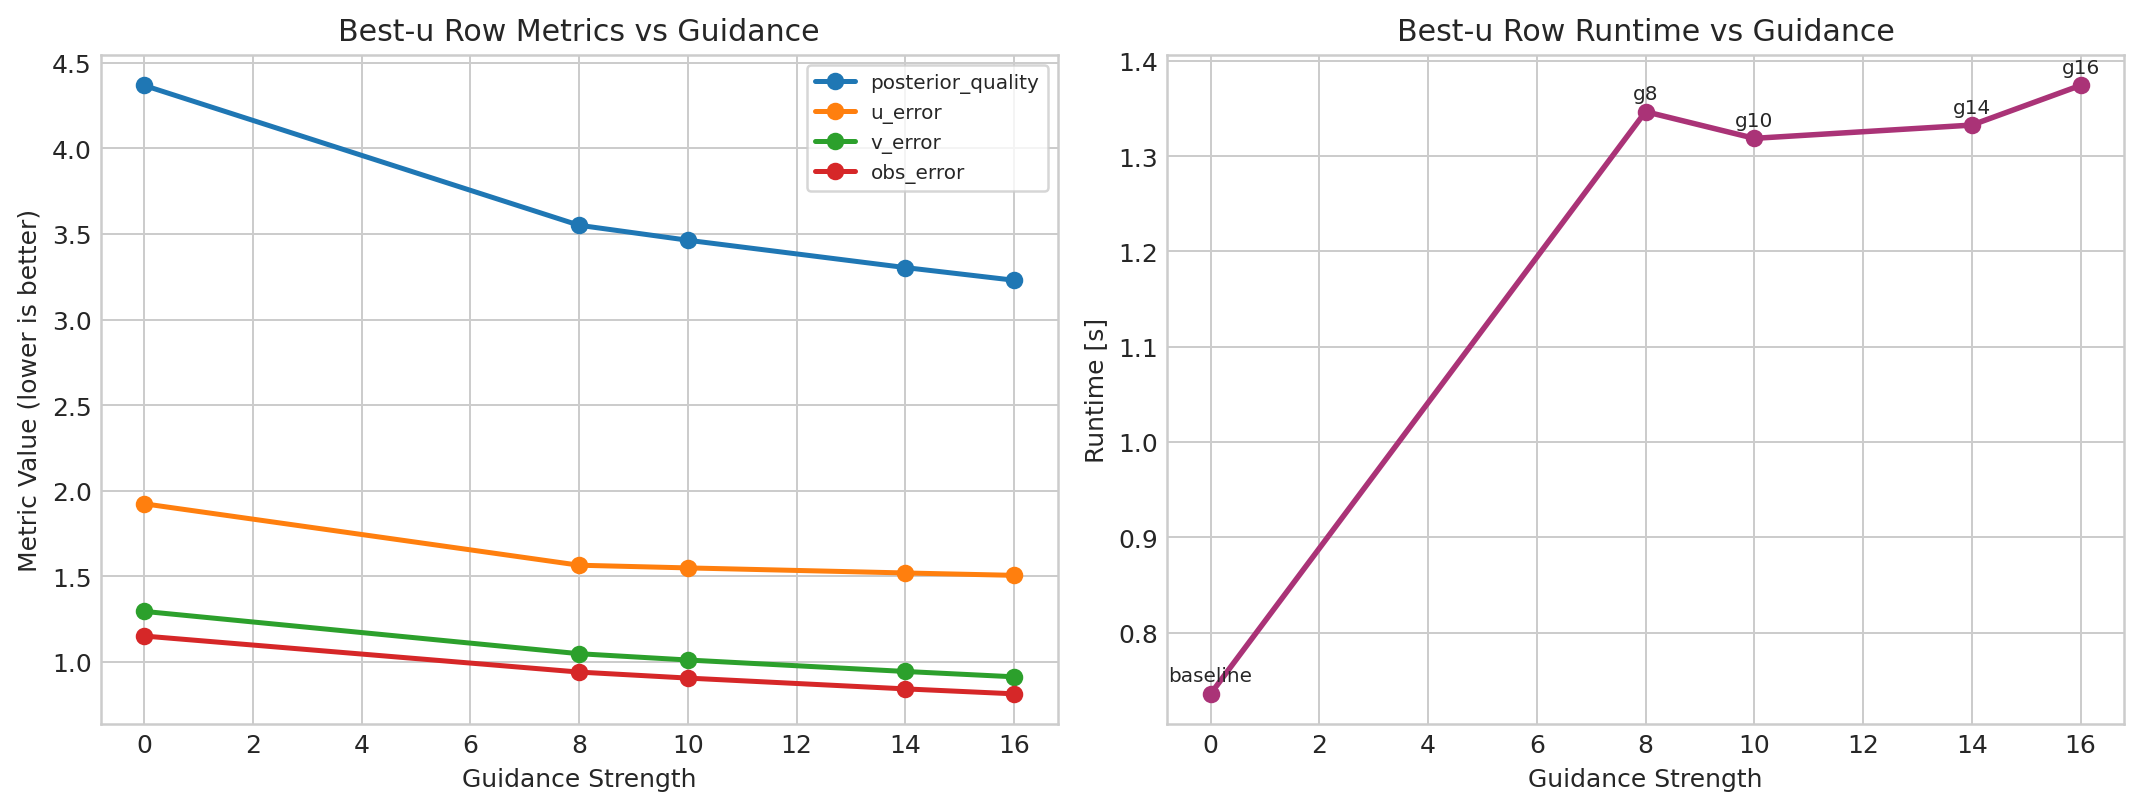
\includegraphics[width=0.95\linewidth]{figures/guidance_trend_best_u.png}
\end{frame}

\begin{frame}{Runtime--Recovery Tradeoff Across Guidance Levels}
\centering
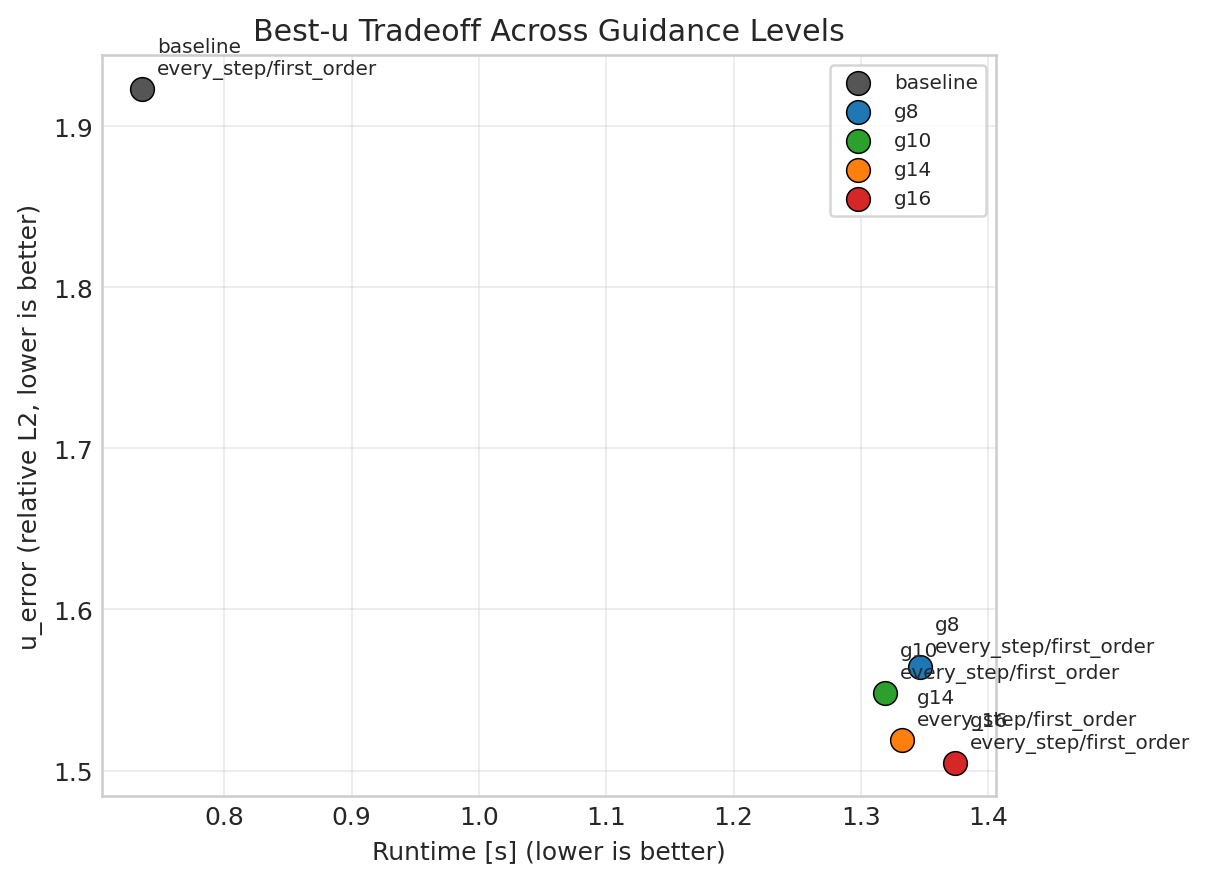
\includegraphics[width=0.78\linewidth]{figures/runtime_uerror_tradeoff.png}
\end{frame}

\begin{frame}{Within \(g=16\): Schedule/Order Tradeoff Map}
\centering
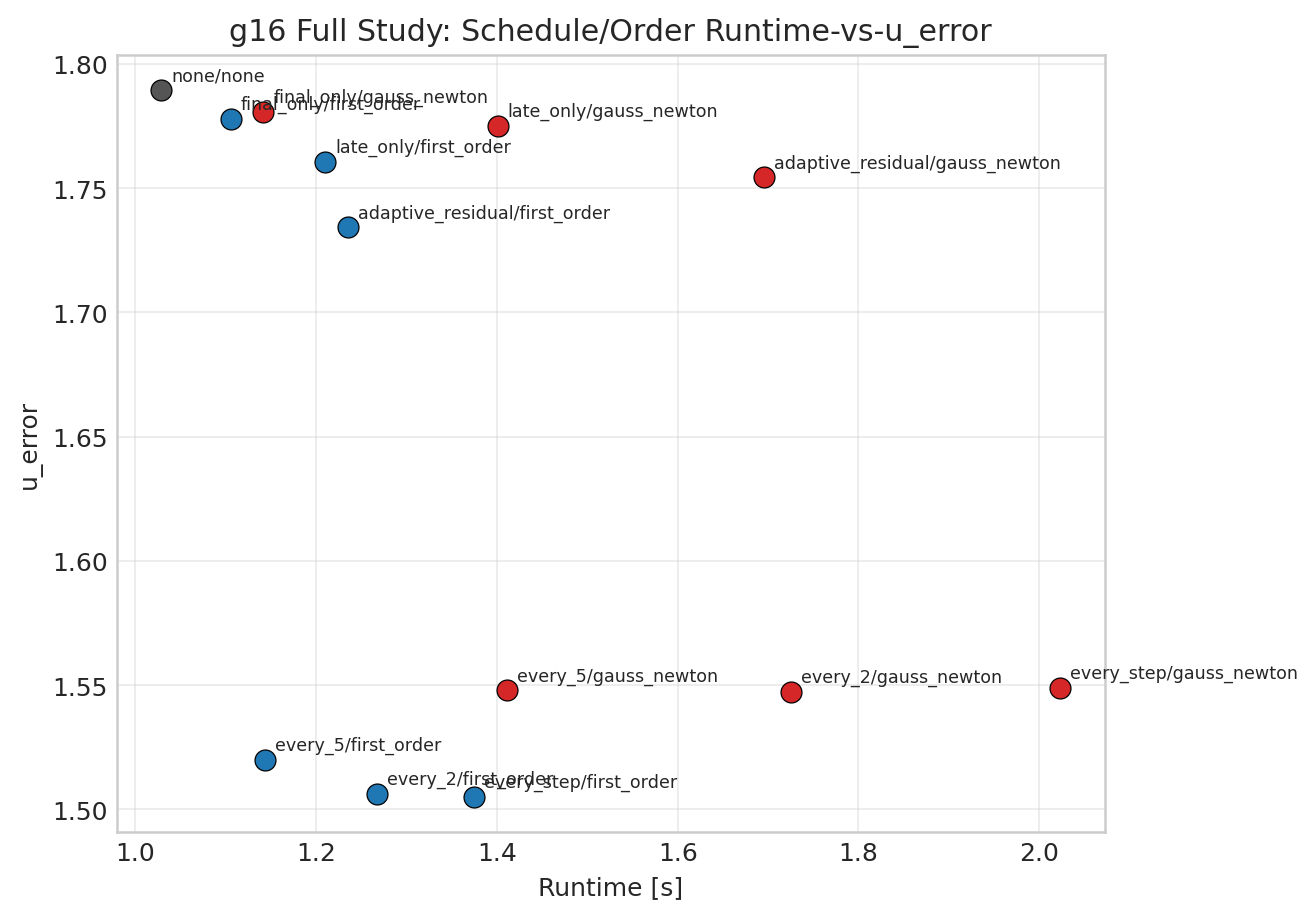
\includegraphics[width=0.82\linewidth]{figures/g16_schedule_tradeoff.png}
\end{frame}

\begin{frame}{Implications and Final Recommendation}
\small
\begin{block}{Do different objectives prefer different projection strategies?}
\textbf{Yes.}
\begin{itemize}
  \item Recovery-focused (\(u\_error\), posterior\_quality): frequent projection, usually \texttt{every\_step / first\_order}.
  \item Physics-focused (\(\|r\|_2\)): \texttt{gauss\_newton} with aggressive projection.
  \item Runtime and trajectory stability: \texttt{none / none}.
\end{itemize}
\end{block}

\begin{block}{Recommended default for inverse posterior recovery}
\texttt{outputs/posterior\_projection\_e200\_big/best.pt} with
\[
\texttt{--observation-guidance-strength }16.0,\quad
\texttt{--num-steps }100,\quad
\texttt{every\_step / first\_order}.
\]
This gives materially better posterior recovery than baseline and than the previous \(g=10\) full-study best.
\end{block}
\end{frame}

\end{document}
